% !TeX root = sm.tex
% !TeX program = latexmk
\documentclass[5p,times]{elsarticle}

\usepackage[T1]{fontenc}
\usepackage[utf8]{inputenc}
\usepackage{microtype}
\usepackage{amsmath,amssymb}
\usepackage{array}
\usepackage{booktabs}
\usepackage{graphicx}
\usepackage{algorithm}
\usepackage{algpseudocode}
\usepackage{pgfplots}
\usepackage{pgfplotstable}
\usepackage{xcolor}
\usepackage[hyphens]{url}
\usetikzlibrary{positioning,arrows.meta,shapes.geometric,calc}
\usepgfplotslibrary{groupplots}
\usepackage[colorlinks=true,linkcolor=blue,citecolor=blue,urlcolor=blue]{hyperref}

\pgfplotsset{compat=1.18}
\usepackage{tabularx}
\newcolumntype{Y}{>{\raggedright\arraybackslash}X}

\definecolor{SNNBlue}{RGB}{31,119,180}
\definecolor{TEOrange}{RGB}{255,127,14}
\definecolor{ECMPGreen}{RGB}{44,160,44}
\definecolor{BanditRed}{RGB}{214,39,40}
\definecolor{BaselineGray}{RGB}{120,120,120}
\definecolor{MemoryPurple}{RGB}{148,103,189}
\definecolor{FullTeal}{RGB}{23,190,207}

\biboptions{numbers,sort&compress}
\emergencystretch=3em
\makeatletter
\def\ps@pprintTitle{%
  \let\@oddhead\@empty
  \let\@evenhead\@empty
  \let\@oddfoot\@empty
  \let\@evenfoot\@empty}
\makeatother

\pgfplotsset{
ieeeplot/.style={
width=\columnwidth,
height=0.68\columnwidth,
tick label style={font=\footnotesize},
label style={font=\footnotesize},
legend style={font=\footnotesize, draw=none, fill=none},
title style={font=\footnotesize},
grid=both,
major grid style={draw=black!12},
minor grid style={draw=black!6},
ymajorgrids=true,
xmajorgrids=false,
line width=0.95pt,
mark size=2.2pt,
},
ieeebar/.style={
ybar,
bar width=8pt,
enlarge x limits=0.18,
nodes near coords={\pgfmathprintnumber[fixed,precision=2]{\pgfplotspointmeta}},
every node near coord/.append style={font=\scriptsize, rotate=90, anchor=west, /pgf/number format/fixed},
},
}

\begin{document}
\begin{frontmatter}
\title{Supplementary Material for NEURA: Local Excitable Routing Control for Stress-Adaptive Networks}
\author[zky]{Haoming Guo}
\author[xidian]{Zhiyuan Ren}
\author[xidian]{Yuehan Li}
\author[xidian]{Wenchi Cheng}
\address[zky]{Institute of Software, Chinese Academy of Sciences, Beijing 100190, China}
\address[xidian]{School of Telecommunications Engineering, Xidian University, Xi'an 710071, China}
\end{frontmatter}

\section{Additional Service and Safety Results}

This supplementary material provides the supporting evidence chain for the low-amplification operating point studied in the main paper. It reports additional startup, path-stretch, gray-failure, safety, mechanism-attribution, and parameter-sensitivity results. Together, these results connect the main delivery-control tradeoff to startup usability, bounded detours, routing-safety indicators, mechanism roles, and parameter robustness.

\subsection{Startup Convergence and Path Stretch}

\begin{figure*}[t]
\centering
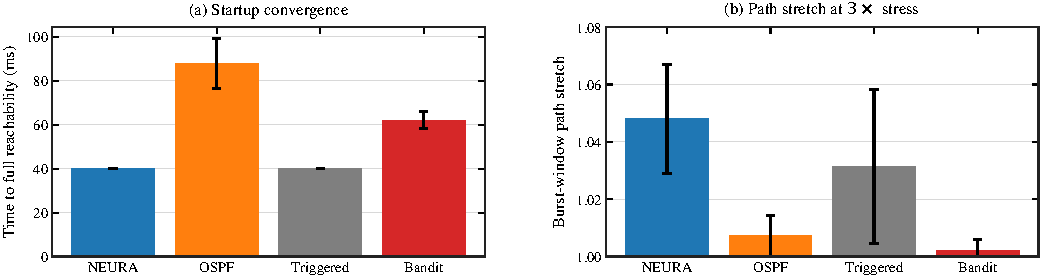
\includegraphics[width=\textwidth]{figures/generated/fig4_startup_and_stretch.pdf}
\caption{Startup cost and data-plane path penalty. Panel (a) reports the time needed to establish full reachability from startup. Panel (b) reports mean burst-window path stretch at the representative $3\times$ hotspot workload. NEURA matches the fastest startup convergence and maintains bounded path inflation rather than achieving low control traffic by allowing arbitrarily poor routes.}
\label{fig:startup-and-stretch}
\end{figure*}


The startup and stretch experiment examines two related questions: how much startup convergence is required before the network becomes fully reachable, and whether the low-overhead operating point is obtained by inflating data-plane routes. Fig.~\ref{fig:startup-and-stretch} reports startup convergence together with burst-window path stretch at the representative $3\times$ hotspot workload.

NEURA reaches full reachability in $40$~ms on average, faster than $88$~ms for OSPF-TE and $62$~ms for Bandit, and matching Triggered-TE at $40$~ms. Its startup control budget is also lower, averaging about $1.76$~MB before full reachability, compared with $2.73$~MB for OSPF-TE, $3.36$~MB for Triggered-TE, and $3.22$~MB for Bandit. Under the representative $3\times$ hotspot workload, NEURA reaches a mean burst-window path stretch of about $1.048$, compared with $1.007$ for OSPF-TE, $1.031$ for Triggered-TE, and $1.002$ for Bandit. These results show that the low-amplification operating point retains fast startup usability and avoids excessive route inflation.

\subsection{Gray-Failure Validation}

The gray-failure validation keeps the topology unchanged and instead degrades the egress service rate of one transit node to $30\%$ of nominal capacity for $300$~ms. This scenario tests whether queue-derived local stress is sufficient to trigger route adaptation without a hard link-down event.

\begin{table}[h]
\centering
\footnotesize
\caption{Gray-failure validation. The impaired transit node remains connected while its egress service rate is reduced to $30\%$ of nominal capacity for $300$~ms.}
\label{tab:gray-failure}
\setlength{\tabcolsep}{3pt}
\renewcommand{\arraystretch}{1.05}
\begin{tabular}{lccc}
\toprule
Method & \shortstack{Delivery\\(\%)} & \shortstack{Ctrl./epoch\\(KB)} & \shortstack{Total ctrl.\\(MB)} \\
\midrule
NEURA & 92.5 & 20.3 & 6.39 \\
Triggered-TE & 96.4 & 329.3 & 41.68 \\
OSPF-TE & 97.3 & 378.3 & 44.53 \\
Bandit & 97.1 & 630.7 & 74.43 \\
\bottomrule
\end{tabular}
\end{table}

NEURA reaches a mean impairment-window delivery ratio of $92.5\%$, lower than the stronger engineering and learning-based baselines, but it does so with a sharply reduced control budget. Triggered-TE closes much of the service gap, but its control budget remains far closer to the periodic baseline than to NEURA. These results support the interpretation that queue-derived local stress is sufficient to trigger useful adaptation under gray failure while preserving the low-control operating point.

\subsection{Safety Indicators}

Table~\ref{tab:safety} separates routing-correctness effects from the control/service tradeoff. The reported values are computed after each method first reaches full pairwise reachability. Pairwise reachability measures whether each source destination pair has at least one usable forwarding chain at the observation instant. The node-complete-route ratio is stricter: it measures the fraction of nodes whose forwarding table contains a currently valid next hop for every destination after local validity checks. A low complete-route ratio can therefore coexist with high burst-window delivery when the missing or stale entries do not lie on the active traffic demands. For NEURA and the stronger periodic, multipath, and learning baselines, final pairwise reachability returns to $100\%$ in these representative runs and the final node-complete-route ratio also returns to $100\%$.

\begin{table*}[t]
\centering
\scriptsize
\caption{Post-startup safety indicators on ER-100 across five seeds. Values report the worst case over seeds after full reachability is first established. Complete-route ratio is a stricter forwarding-table completeness metric than pairwise reachability.}
\label{tab:safety}
\setlength{\tabcolsep}{16pt}
\renewcommand{\arraystretch}{1.05}
\begin{tabular}{llccccc}
\toprule
Scenario & Method &
\shortstack[c]{Worst post-startup\\reach. (\%)} &
\shortstack[c]{Worst\\loop (\%)} &
\shortstack[c]{Worst\\blackhole (\%)} &
\shortstack[c]{Worst final\\reach. (\%)} &
\shortstack[c]{Worst final\\complete-route (\%)} \\
\midrule
Hotspot $3\times$ & NEURA & 99.87 & 0.13 & 0.00 & 100.0 & 100.0 \\
Hotspot $3\times$ & Triggered-TE & \textbf{98.97} & \textbf{1.03} & 0.00 & \textbf{99.05} & \textbf{6.0} \\
Hotspot $3\times$ & OSPF-TE & 99.88 & 0.12 & 0.08 & 100.0 & 100.0 \\
Hotspot $3\times$ & TE+ECMP & 99.92 & 0.00 & 0.08 & 100.0 & 100.0 \\
Hotspot $3\times$ & Bandit & 99.96 & 0.00 & 0.04 & 100.0 & 100.0 \\
Continuous chaos & NEURA & 99.87 & 0.13 & 0.00 & 100.0 & 100.0 \\
Continuous chaos & Triggered-TE & \textbf{97.64} & \textbf{2.36} & 0.00 & \textbf{99.02} & \textbf{3.0} \\
Continuous chaos & OSPF-TE & 99.88 & 0.12 & 0.08 & 100.0 & 100.0 \\
Continuous chaos & TE+ECMP & 99.92 & 0.00 & 0.08 & 100.0 & 100.0 \\
Continuous chaos & Bandit & 99.96 & 0.00 & 0.04 & 100.0 & 100.0 \\
Gray failure & NEURA & 99.94 & 0.06 & 0.00 & 100.0 & 100.0 \\
Gray failure & Triggered-TE & \textbf{99.11} & \textbf{0.89} & 0.00 & \textbf{99.12} & \textbf{13.0} \\
Gray failure & OSPF-TE & 99.92 & 0.00 & 0.08 & 100.0 & 100.0 \\
Gray failure & TE+ECMP & 99.92 & 0.00 & 0.08 & 100.0 & 100.0 \\
Gray failure & Bandit & 99.96 & 0.00 & 0.04 & 100.0 & 100.0 \\
\bottomrule
\end{tabular}
\end{table*}

The nearest-neighbor Triggered-TE baseline is the main exception. It preserves strong burst-window delivery in the main service figures, but its post-startup reachability floor drops under the representative hotspot and continuous-chaos workloads, and its worst final node-complete-route ratio is much lower than the other baselines. This does not mean that Triggered-TE is unusable in the service-window measurements; it means that, under the stricter all-destinations table-completeness check, some inactive or noncritical destination entries remain stale or invalid after stress. By contrast, the main NEURA tradeoff is not explained by persistent loops, blackholes, or incomplete forwarding-table recovery.

\section{Mechanism Attribution}

The mechanism attribution study asks which parts of the control law are responsible for the observed operating point. Table~\ref{tab:neura-ablation} combines two targeted studies that use the same routing engine but isolate different failure modes of the control plane.

The top row studies rebound after a two-stage disturbance. In the minimal event-driven core without memory, the rebound ratio after release is about $1.57\%$ and the system continues to accumulate about $21$ post-stage-2 route changes. Adding memory alone reduces the rebound ratio to about $1.40\%$ and eliminates post-stage-2 route changes. The full mechanism lowers the rebound ratio further to about $0.28\%$ while also reducing total emitted updates from about $208$k to about $166$k over the same run.

The bottom row studies switch suppression inside the queue-closed-loop continuous-chaos workload. Removing the switch-suppression terms increases route rewrites from about $100$ to about $126$ per node and raises the peak event rate from about $29.7$k to about $41.6$k messages per tick. Mean burst delivery remains slightly higher without switch suppression, which clarifies the role of this mechanism: it suppresses excessive local switching and prevents a stressed region from turning into a sharper control-plane burst.
\begin{table}[h]
\centering
\scriptsize
\caption{Mechanism attribution for NEURA. Panel A isolates rebound suppression, and Panel B isolates burst containment. Bold entries mark the decisive attribution values discussed in the text.}
\label{tab:neura-ablation}
\renewcommand{\arraystretch}{1.05}
\begin{tabular*}{\columnwidth}{@{\extracolsep{\fill}}lcccc@{}}
\toprule
Variant & \shortstack[c]{Del.\\(\%)} & \shortstack[c]{Rebound\\(\%)} & \shortstack[c]{Post-stage-2\\changes} & \shortstack[c]{Updates\\(k)} \\
\midrule
\multicolumn{5}{@{}l}{\textbf{A. Rebound suppression}} \\
\cmidrule(lr){1-5}
Minimal core & 96.0 & 1.57 & \textbf{21.0} & 208.4 \\
Memory only & 96.0 & 1.40 & 0.0 & 180.8 \\
Full NEURA & 96.0 & \textbf{0.28} & 0.0 & 165.5 \\
\midrule
Variant & \shortstack[c]{Burst del.\\(\%)} & \shortstack[c]{Route chg.\\per node} & \shortstack[c]{Peak rate\\($10^3$/tick)} & \shortstack[c]{Loss\\ticks} \\
\midrule
\multicolumn{5}{@{}l}{\textbf{B. Burst containment}} \\
\cmidrule(lr){1-5}
Full NEURA & 96.0 & 100.1 & 29.7 & 7.4 \\
No memory & 96.0 & 100.0 & 29.7 & 7.4 \\
No switch supp. & 96.7 & \textbf{125.9} & \textbf{41.6} & 8.0 \\
No slow state & 96.0 & 100.1 & 29.7 & 7.4 \\
\bottomrule
\end{tabular*}
\end{table}


\section{Parameter Sensitivity}

The focused sensitivity study indicates that the reported operating point lies inside a usable tested neighborhood. Threshold $\theta$ and refractory duration $T_{\mathrm{ref}}$ form the clearest response-versus-overhead tradeoff. Increasing $\theta$ from $1.1$ to $1.7$ changes the mean burst-delivery ratio from $0.925$ to $0.913$ while reducing mean total emitted updates from $2.36\times 10^5$ to $1.78\times 10^5$. Increasing $T_{\mathrm{ref}}$ from $2$ to $6$ keeps the mean burst-delivery ratio near $0.923$ to $0.926$ while reducing mean total emitted updates from $2.24\times 10^5$ to $1.62\times 10^5$.

The memory-retention and slow-timescale sweeps are comparatively stable in the tested region. Varying $\eta$ from $0.55$ to $0.90$ changes the mean burst-delivery ratio only from $0.924$ to $0.922$, and varying $\omega_s$ from $0.15$ to $0.55$ changes it only from $0.923$ to $0.923$. In the repeated-disturbance sensitivity sweep, post-stage-2 route changes remain saturated at zero across the tested values.

\begin{table}[t]
\centering
\scriptsize
\caption{Sensitivity-summary of the main control parameters in NEURA. The table reports the dominant trend observed over each sweep rather than the full sampled matrix.}
\label{tab:sensitivity-summary}
\renewcommand{\arraystretch}{1.05}
\begin{tabularx}{\columnwidth}{@{}l c >{\raggedright\arraybackslash}X >{\raggedright\arraybackslash}X@{}}
\toprule
Parameter & Range & Main effect & Interpretation \\
\midrule
$\theta$ & $1.1$--$1.7$ &
Delivery $0.925\!\rightarrow\!0.913$; updates $2.36\times10^5\!\rightarrow\!1.78\times10^5$ &
Higher threshold lowers control overhead at a modest service cost \\

$T_{\mathrm{ref}}$ & $2$--$6$ &
Delivery nearly unchanged; updates $2.24\times10^5\!\rightarrow\!1.62\times10^5$ &
Temporal suppression effectively reduces control activity \\

$\eta$ & $0.55$--$0.90$ &
Delivery changes only from $0.924$ to $0.922$ &
Memory retention is stable in the tested region \\

$\omega_s$ & $0.15$--$0.55$ &
Delivery remains essentially unchanged at $0.923$ &
Slow state acts as a secondary stabilizer rather than a main lever \\

$g_0$ & $0.25$--$0.65$ &
Delivery $0.925\!\rightarrow\!0.923$; chaos control $7.94\!\rightarrow\!8.11$ MB &
Stable operating region under moderate guard variation \\

$g_1$ & $0.15$--$0.55$ &
Route changes $110\!\rightarrow\!101$; delivery $0.928\!\rightarrow\!0.918$ &
A smooth churn--service knob \\

$w_n$ & $0.2$--$0.5$ &
Reducing $w_n$ to $0.2$ lowers delivery to $0.887$ &
Explicit next-hop stress awareness is important \\

TTL & $4$--$12$ &
No measurable effect &
No measurable effect in the tested locality range \\
\bottomrule
\end{tabularx}
\end{table}

\end{document}
